% !TEX TS-program = pdflatex

\documentclass[unicode,11pt,notheorems,xcolor=table]{beamer}
\usepackage{fix-cm}
\usepackage[T2A]{fontenc}
\usepackage[utf8]{inputenc}
\usepackage[russian]{babel}
\usepackage{amsmath,amsfonts,amssymb,amsthm}
\usepackage{mathtools}
\usepackage{diagbox}

\usepackage{ulem}
\usepackage{tikz}
\usepackage{graphicx}
\usepackage{pgfplots}
\pgfplotsset{compat=1.16}

\usetikzlibrary{matrix,arrows,decorations.pathmorphing, arrows.meta,positioning}
\usetikzlibrary{positioning,calc}
\usetikzlibrary{patterns}
\usetikzlibrary{decorations.pathreplacing}

%Описание стиля презентации
\usetheme[sidebar=0]{kfmn} 
\setbeamercovered{transparent}

%\definecolor{cyan}{RGB}{240,217,1}
%\definecolor{vgugreen}{RGB}{143,188,103}
%\definecolor{vgured}{RGB}{234,38,40}
%\definecolor{vgublue}{RGB}{53,101,167}
\hypersetup{colorlinks,linkcolor=,urlcolor=blue}

\makeatletter
	\g@addto@macro{\endtabular}{\rowfont{}}% Clear row font
	\makeatother
	\newcommand{\rowfonttype}{}% Current row font
	\newcommand{\rowfont}[1]{% Set current row font
		\gdef\rowfonttype{#1}#1\ignorespaces%
	}
\makeatother

\newcommand{\myunit}{9mm}
\tikzset{
    node style sp/.style={draw,circle,minimum size=\myunit},
    node style ge/.style={circle,minimum size=\myunit},
    arrow style mul/.style={draw,sloped,midway,fill=white},
    arrow style plus/.style={midway,sloped,fill=white},
}

%[0, 6, 8, 8, 10, 5, 6, 10, 8, 10, 10], 

\pgfdeclareimage[height=8mm]{university-logo}{logo-iem.png}
\logo{\pgfuseimage{university-logo}}
%2[0, 11, 10, 8, 11, 5, 11, 11, 8, 11, 10, 11],

\titlepicture{
	\begin{tikzpicture}[y=1.4cm,overlay,rotate=8]
	\coordinate (O) at (-3cm,0.9cm);
	\filldraw[thick,draw= vgublue, fill=vgublue!20!white] (0,0) circle[radius=4.2cm];
	\clip (0,0) circle[radius=4.2cm];
	\draw (-1.5,1.5) node{
	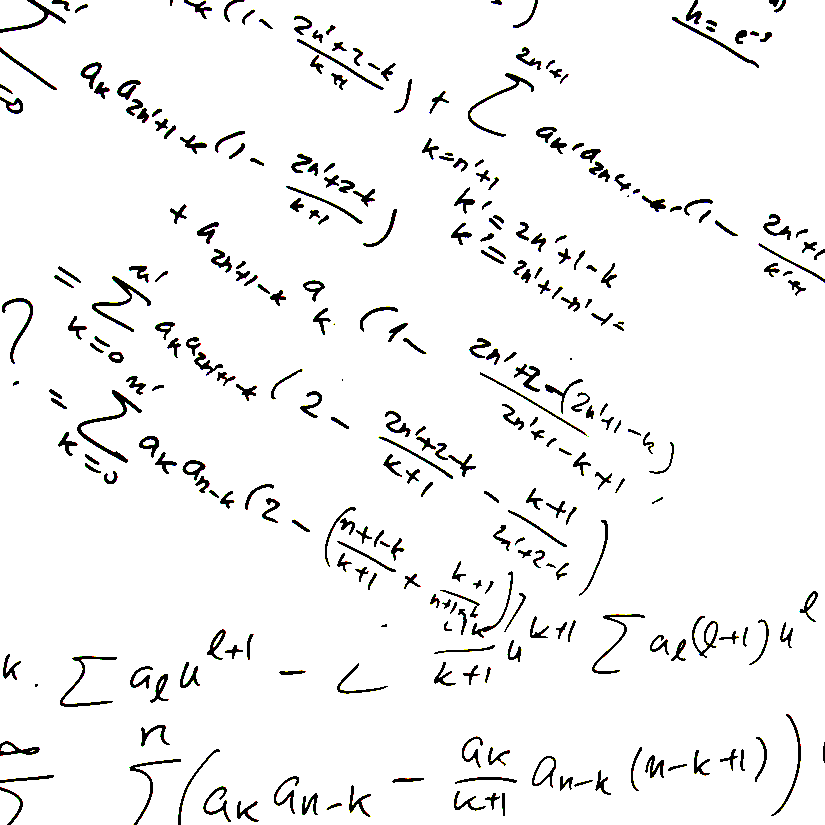
\includegraphics[width=8cm]{titlepic.png}
	};
\end{tikzpicture}
}

\usepackage[math]{iwona}

\newcommand{\hplus}{\mathbin{\hat+}}
\newcommand{\hdot}{\mathbin{\hat\cdot}}
% Описание теорем
\newtheorem{theorem}{Теорема}
\newtheorem{seq}{Следствие}
%%

\LECT % 

% Титульный лист теорем
\author[Д.\,В. Чупраков]{канд.\,физ.-матем.\,наук, доцент Д.\,В. Чупраков\\[6pt] usr10381@vyatsu.ru}

\institute[ВятГУ]{ФГБОУ ВО Вятский государственный университет}

\department{Факультет экономики и финансов}

\title[Лекция~19. Проверка гипотез -- 2]{
	Введение в экономико-математическое моделирование\\[12pt]
	Лекция~19. Проверка гипотез}
\date{9 декабря 2020~г.}


\setbeamercovered{invisible}

\setbeamercolor{math text}{fg=vgured!70!black}

\pgfmathdeclarefunction{gauss}{2}{%
  \pgfmathparse{1/(#2*sqrt(2*pi))*exp(-((x-#1)^2)/(2*#2^2))}%
}
\begin{document}


\maketitle

 \begin{frame}{Структура лекции}{}
 	\tableofcontents
 \end{frame}

\section{}

\begin{frame}{Статистическая гипотеза}{}

    \begin{block}{Определеине}
    \alert{Статистическая гипотеза}
    это предположение
    \begin{itemize}
        \item о виде распределения генеральной совокупности или 
        \item о величинах неизвестных параметров известного распределения генеральной совокупности,
    \end{itemize}
    которое может быть проверено на основании выборочных показателей.
    \end{block}

    По количеству предположений гипотезы делятся на:
    \begin{itemize}
        \item простые~--- это гипотезы, содержащие только одно предположение;
        \item сложные~--- гипотезы, состоящие из конечного или бесконечного числа простых гипотез.    
    \end{itemize}
\end{frame}
    % Проверка статистической гипотезы заключается в сопоставлении некоторых статистических показателей, вычисленных по данным выборки со значениями этих же показателей, определенных теоретически в предположении, что проверяемая гипотеза верна.



\begin{frame}{Mortal Combat}{}

\includegraphics[width=\textwidth]{vs.png}

\bigskip
\section{Понятие статистической гипотезы}

\begin{minipage}{5cm}
    \structure{Нулевая гипотеза $\color{vgublue} H_0$}~--- 
    
    гипотеза, подлежащая проверке. 
    
\end{minipage}
\hfill
\begin{minipage}{5cm}
\alert{Конкурирующая (альтернативная) гипотеза}~$H_1$~--- 

любое утверждение, которое противоречит нулевой гипотезе.    
\end{minipage}

\end{frame}


\begin{frame}{Нулевая гипотеза}{}
    Нулевая гипотеза~--- утверждение, принимаемое по умолчанию.

    \vfill

    Проверяя статистическую гипотезу исследователь пытается показать несостоятельность нулевой гипотезы, несогласованность её с имеющимися опытными данными, то есть отвергнуть гипотезу. 

    \vfill

    При этом подразумевается, что должна быть принята другая, альтернативная (конкурирующая), исключающая нулевую гипотезу. 

    \vfill

    Отвергнуть нулевую гипотезу~--- значит сделать вывод, что  \alert{конкурирующая гипотеза $H_1$ лучше описывает реальность, чем нулевая гипотеза $H_0$}
\end{frame}


\begin{frame}{Презумпция невиновности}{}

    Для нулевой гипотезы действует своеобразная ,,презумпция невиновности``':

    \begin{block}{}
        Нулевая гипотеза считается верной, пока не будет доказано обратное (нулевая гипотеза отвергнута) сверх необходимых сомнений (т.\,е. в статистически значимой степени).
    \end{block}

    \vfill

    Истинность нулевой гипотезы невозможно доказать, но можно показать, что в данный момент нет причин сомневаться в ней.


    % Рассмотрим 
    % 
    % Например о том
    % предположение о том, что не существует связи между двумя наблюдаемыми событиями, феноменами. Так, нулевая гипотеза считается верной до того момента, пока нельзя доказать обратное. 
%     Опровержение нулевой гипотезы, то есть приход к заключению о том, что связь между двумя событиями, феноменами существует, — главная задача современной науки. 
%     Статистика как наука даёт чёткие условия, при наступлении которых нулевая гипотеза может быть отвергнута.

% Часто в качестве нулевой гипотезы выступают предположения об отсутствии взаимосвязи или корреляции между исследуемыми переменными, об отсутствии различий (однородности) в распределениях (параметрах распределений) в двух и/или более выборках. Для обозначения нулевой гипотезы часто используют символ H0.

%
\end{frame}


\section{Статистический критерий}

\begin{frame}{Статистический критерий}{}
    \begin{block}{}
        \alert{Статистический критерий}~--- правило, которое позволяет на основе имеющихся данных отвергнуть нулевую гипотезу. 
    \end{block}
    \bigskip
    \begin{itemize}
        \item \alert{Параметрические}~--- критерии, которые служат для проверки гипотез о параметрах распределений генеральной совокупности (чаще всего нормального распределения).
        \item \alert{Непараметрические} - критерии, которые для проверки гипотез не используют предположений о распределении генеральной совокупности. Эти критерии не требуют знания параметров распределений.
        \item \alert{Критерии согласия}~---  служат для проверки гипотез о согласии распределения генеральной совокупности, из которой получена выборка, с ранее принятой теоретической моделью (чаще всего нормальным распределением).
    \end{itemize}
    
\end{frame}


\begin{frame}{Статистика критерия}{}
    В основе критерия лежит \alert{статистика критерия}~---
    искусственно сконструированная функция
    $$
        T_n=T(X_1,X_2, \ldots, X_n)
    $$
    от выборки
    $X_1,X_2, \ldots, X_n$.

    \bigskip
    \begin{block}{}
        \begin{itemize}
            \item Статистика критерия  является случайной величиной.
            \item \alert{Закон распределения статистики критерия должен быть известнен!}
        \end{itemize}
    \end{block}

\end{frame}

\begin{frame}{Обозначение статистики}{}
    В зависимости от закона распределения статистику обозначают через: 
    \begin{itemize}
        \item $U$ или $Z$, если она имеет нормальное распределение; 
        \item $F$ или $v^2$~---  распределение Фишера; 
        \item $\chi^2$~--- распределение «хи квадрат»;  
        \item $t$~--- распределение Стьюдента.
    \end{itemize}
\end{frame}

\begin{frame}{Критическая область}{}
    Множество всех значений статистики критерия 
    разбивается на два непересекающихся подмножества:
    \begin{itemize}
        \item \alert{Критическую область}~--- включает значения статистики, появление которых при справедливости $H_0$ практически невозможно.
        \item \alert{Область допустимых значений (область принятия гипотезы)}~--- значения которые может принимать статистика при условии справедливости нулевой гипотезы~$H_0$;
    \end{itemize}

    \bigskip
    \hrule
    \bigskip

    \begin{itemize}
        \item  Статистика подбирается так, чтобы область допустимых значений и критическая область были интервалами.

        \item Вид критической области зависит от типа альтернативной гипотезы.
    \end{itemize}
\end{frame}

\begin{frame}{Отвержение и принятие гипотезы}{}
    \begin{alertblock}{Условие отвержения гипотезы}
        Если значение статистики попадает в критическую область, то гипотеза $H_0$ отвергается в пользу альтернативной.
    \end{alertblock}

    \vspace{15mm}
    
    \begin{exampleblock}{Условие согласия гипотезы}
        Если значение статистики попадает в область допустимых значений, то гипотеза $H_0$ не противоречит наблюдаемым значениям, поэтому нет оснований отвергать ее.

        \vspace{5mm}
        \alert{Нулевая гипотеза принимается только волевым решением исследователя.}
    \end{exampleblock}
\end{frame}


%TODO Пример про беременного мужика.

\begin{frame}{Матрица ошибок}{}
\begin{tabular}{|>{\columncolor{vgublue}}l|m{35mm}|m{35mm}|}
    \hline
    \rowcolor{vgublue}& $\color{white} H_0$ \color{white}  верна & $\color{white} H_0$ \color{white} неверна\\
    \hline
    $\color{white} H_0$ \color{white} принята & Верное решение &  \cellcolor{red!30} Ошибка II рода \\ 
    \hline
    $\color{white} H_0$ \color{white} отвергнута & \cellcolor{red!30}  Ошибка I рода &  Верное решение\\ 
    \hline
\end{tabular}   

\vfill
\begin{itemize}
    \item \alert{Ошибка первого рода}~--- отвержение верной гипотезы $H_0$.
    \item \alert{Ошибка второго рода}~--- принятие ошибочной гипотезы $H_0$.
\end{itemize}

\vfill

% Какая из ошибок является более опасной, зависит от конкретной задачи.

\vfill
{\centering
\begin{tikzpicture}
   \begin{axis}[
     name=myaxis,
     no markers, domain=-2:4, samples=500,
     axis y line=none,
     axis x line=center,
     xlabel=$T$, %ylabel=$p$,
      every axis y label/.style={at=(current axis.above origin),anchor=south},
      every axis x label/.style={at=(current axis.right of origin),anchor=west},
      height=5cm, width=11cm,
      xmin=-2.1, xmax=4.1,
      ymin=-0.1, ymax=0.5,
      xtick=\empty, ytick=\empty,
      enlargelimits=false, clip=false, axis on top,
     grid = none
     ]
    \addplot [fill=cyan!20, draw=none, domain=1.4:3] {gauss(0,1)} \closedcycle;
    \addplot [fill=red!20, draw=none, domain=0:1.4] {gauss(3,1)} \closedcycle;
    \addplot [very thick,cyan!50!black] {gauss(0,1)};
    \addplot [very thick,red!50!black] {gauss(3,1)};
          
    \draw[thick,vgured!50, rounded corners = 4mm] (axis cs:4,-0.05) -| (axis cs:1.4,0);
    \draw[thick,cyan!50, rounded corners = 4mm] (axis cs:-2,-0.05) -| (axis cs:1.4,0);

    % \fill[cyan!20] (axis cs:1.4,-0.02) rectangle (axis cs:-2,0);

    \node[coordinate,pin=135:{Ошибка II рода}]
       at (axis cs:1.2,0.02) {};
       \node[coordinate,pin=45:{Ошибка I рода}]
       at (axis cs:1.6,0.04) {};
    \draw[vgured] (axis cs:1.4,-0.04) node[below]{$T_\text{кр.}$} -- (axis cs:1.4,0.5);
    \end{axis}
   \end{tikzpicture}
   \par}      


% При разработке статистического критерия невозможно одновременно минимизировать обе ошибки. 
    
% Поэтому поступают следующим образом: при заданном числе испытаний n устанавливается верхняя граница для ошибки первого рода 
% Выбирается тот критерий, у которого наименьшая ошибка второго рода.

\end{frame}

\begin{frame}{Уровень значимости}{}
    
    \begin{block}{Определеине}
        Вероятность ошибки первого рода называется \alert{уровнем значимости $\alpha$}.
    \end{block}
    \
    Уровень значимости $\alpha$ устанавливается из значений следующего ряда:
    $$
        0.05,\quad 0.01,\quad 0.005,\quad \ldots
    $$
    события с такими вероятностями считаются практически невозможными.

    Допустимая величина уровня значимости определяется теми последствиями, которые наступают после совершения ошибки.
\end{frame}

\begin{frame}{Критическое значение}{}
    
    Так как область допустимых значений и критическая область являются интервалами, то существует граничная точка, разделяющая их

    {\centering
    \begin{tikzpicture}
       \begin{axis}[
         name=myaxis,
         no markers, domain=-3:3, samples=500,
         axis y line=center,
         axis x line=center,
         xlabel=$T$, %ylabel=$p$,
          every axis y label/.style={at=(current axis.above origin),anchor=south},
          every axis x label/.style={at=(current axis.right of origin),anchor=west},
          height=5cm, width=11cm,
          xmin=-3.1, xmax=3.1,
          ymin=-0.1, ymax=0.5,
          xtick=\empty, ytick=\empty,
          enlargelimits=false, clip=false, axis on top,
         grid = none
         ]
        \addplot [fill=cyan!20, draw=none, domain=1.4:3] {gauss(0,1)} \closedcycle;
        \addplot [very thick,cyan!50!black] {gauss(0,1)};
              
        \fill[vgured!20] (axis cs:1.4,-0.03) rectangle (axis cs:3,0);
        \node[coordinate,pin=-45:{Критическая область}]
           at (axis cs:1.6,-0.02) {};
           \node[coordinate,pin=45:{Уровень значимости $\alpha$}]
           at (axis cs:1.6,0.04) {};
        \draw[vgured] (axis cs:1.4,-0.04) node[below]{$T_\text{кр.}$} -- (axis cs:1.4,0.5);
        \end{axis}
       \end{tikzpicture}
       \par}      
    
    

    \alert{Критическое значение статистики}~--- граница области допустимых значений статистики, при условии, что нулевая гипотеза $H_0$ верна. 

    
    
    % Для того чтобы понять, действительно ли разница между значением параметра в гипотезе и значением оценки, полученной по выборке, является существенной, необходимо сравнить два показателя: 
    % \begin{itemize}
    %     \item наблюдаемое значение статистики и 
    %     \item критическое значение статистики.
    % \end{document}        
    %     Наблюдаемое значение статистики – значение статистики, которое получается по выборке, на основе имеющихся данных.
    %    
        
    %     Критическое значение статистики отделяет область допустимых  значений статистики откритической области области редких значений статистики при условии, что нулевая гипотеза верна. Область типичных значений – область не-отвержения ну-левой гипотезы, критическая область – область отвержения нулевой гипотезы. 
\end{frame}

\begin{frame}{Типы критической области}{}
    \structure{Односторонняя:}
    \begin{itemize}
        \item \alert{Левосторонняя}~--- определяется $P(T< T_\text{кр})=\alpha$

        \medskip
        {\centering
        \begin{tikzpicture}[>=latex]
            \draw[thick,->] (0,0) -- (8,0) node[below]{$T$};
            \fill (4,0) circle[radius=1pt] node[below]{$T_\text{кр}$};
            \draw[rounded corners = 3mm] (0,0.5) -| (4,0);
        \end{tikzpicture}
        \par}

        \item \alert{Правосторонняя}~--- определяется $P(T> T_\text{кр})=\alpha$

        \medskip
        {\centering
        \begin{tikzpicture}[>=latex]
            \draw[thick,->] (0,0) -- (8,0) node[below]{$T$};
            \fill (4,0) circle[radius=1pt] node[below]{$T_\text{кр}$};
            \draw[rounded corners = 3mm] (8,0.5) -| (4,0);
        \end{tikzpicture}
        \par}
        \end{itemize}
        
        \bigskip
        \structure{Двухсторонняя}~--- определяется $P(T> |T_\text{кр}|)=\dfrac{\alpha}{2}$

        \medskip
        {\centering
        \hspace{5mm}
        \begin{tikzpicture}[>=latex]
            \draw[thick,->] (0,0) -- (8,0) node[below]{$T$};
            \fill (3,0) circle[radius=1pt] node[below]{$-T_\text{кр.}$};
            \fill (5,0) circle[radius=1pt] node[below]{$T_\text{кр.}$};
            \draw[rounded corners = 3mm] (0,0.5) -| (3,0);
            \draw[rounded corners = 3mm] (8,0.5) -| (5,0);
        \end{tikzpicture}
        \par}
        
    
\end{frame}

\begin{frame}{Мощность критерия}{}

    \begin{block}{Определеине}
        \alert{Мощность критерия}~---  вероятность попадания критерия в критическую область при условии, что верна конкурирующая гипотеза.
    \end{block}

    \vfill 
    Если $\beta$~--- вероятность ошибки второго рода, то мощность критерия равна $1-\beta$. 
    
    
    \vfill 
    Чем больше мощность критерия, тем меньше вероятность совершить ошибку второго рода. 
    
    \vfill 
    \begin{block}{}
        После выбора уровня значимости~$\alpha$ следует строить критическую область так, чтобы мощность критерия была максимальной.
    \end{block}
\end{frame}

{\setbeamercolor{background canvas}{bg=yellow!10}
\section{Алгоритм проверки гипотез}
\begin{frame}{Алгоритм проверки гипотез}{}
\begin{enumerate}
    \item Формулируются гипотезы $H_0$ и $H_1$.
    \item По виду гипотезы выбирается статистический критерий $T$;
    \item Выбирается уровень значимости критерия $\alpha$. Он равен вероятности допустить ошибку первого рода.
    \item По выборочным данным вычисляется вычисляется наблюдаемое значение сатистики $T_\text{набл.}$
    \item По уровню значимости $\alpha$ вычисляется критическое значение $T_\text{кр}$, разделяющее критическую область и область допустимых значений.
    \item Определяется неравенство, задающее критическую область.
\end{enumerate}

\medskip
\hrule
\medskip

\begin{itemize}
    \item Если $T_\text{набл.}$ попадает в  критическую область, то нулевая гипотеза отвергается.
    \item  Если $T_\text{набл.}$ попадает в область допустимых значений, то нулевая гипотеза не противоречит наблюдаемым данным.
\end{itemize}    
\end{frame}
}

% \section{Проверка гипотезы о вероятности события}
% \begin{frame}{Проверка гипотезы о вероятности события}{}
%     Пусть проведено $n$ независимых испытаний, в каждом из которых некоторое событие $A$ появляется с одной и той же, но неизвестной вероятностью $p$.
    
%     \bigskip
%     Найдена относительная частота $\omega(A)=\frac{m}{n}$ появлений $A$ в этой серии испытаний. 

%     \bigskip
    
%     \begin{block}{Нулевая гипотеза }
%         $H_0\colon$ Вероятность $p$ события $A$ равна некоторому значению $p_0$.
%     \end{block}

% \end{frame}

% \begin{frame}{Статистический критерий}{}

 
%     {\small По теореме Лапласа при достаточно большом $n$ относительную
 
%     частоту можно приближенно считать нормально распределенной с математическим ожиданием $p$ и средним квадратическим
%     отклонением  $\sigma_\omega = \sqrt{\frac{pq}{n}}$, где $q=1-p$. 
%     \par}
    
%     \bigskip

%     \begin{block}{Статистический критерий}
%         \centering
%         $ \displaystyle
%             U=\left(\omega-p_0\right)\frac{\sqrt{n}}{\sqrt{p_0(1-p_0)}} \sim N(0,1)
%         $
%     \end{block}

%     \bigskip
%     Наблюдаемое значение вычисляется по формуле:
%     $$
%         U_\text{набл.}=\left(\frac{m}{n}-p_0\right)\frac{\sqrt{n}}{\sqrt{p_0(1-p_0)}}
%     $$
%     где $n$~--- число испытаний, $m$~--- число появлений события~$A$

 
% \end{frame}

% \begin{frame}{Критическая область гипотезы $H_1\colon p \neq  p_0$}{}
 
%     % Примем уровень значимости~$\alpha$.

%     \begin{itemize}
%             \item Критическая область: \hfill $(-\infty ;-U_\text{кр})\cup (U_\text{кр}; +\infty )$
%             \item Значение $U_\text{кр}$ определяется из условия \hfill 
%             $\Phi(U_\text{кр}) = \dfrac{1-\alpha}{2}$
%             \item Нулевая гипотеза отвергается, если \hfill $|U_\text{набл}| > U_\text{кр}$.
%     \end{itemize}

%     {\centering
%      \begin{tikzpicture}
%         \begin{axis}[
%           name=myaxis,
%           no markers, domain=-3:3, samples=500,
%           axis y line=center,
%           axis x line=center,
%           xlabel=$U$, ylabel=$p$,
%            every axis y label/.style={at=(current axis.above origin),anchor=south},
%            every axis x label/.style={at=(current axis.right of origin),anchor=west},
%            height=5cm, width=11cm,
%            xmin=-3.1, xmax=3.1,
%            ymin=-0.1, ymax=0.5,
%            xtick=\empty, ytick=\empty,
%            enlargelimits=false, clip=false, axis on top,
%           grid = none
%           ]
%           \addplot [fill=cyan!20, draw=none, domain=1.3:3] {gauss(0,1)} \closedcycle;
%           \addplot [fill=cyan!20, draw=none, domain=-3:-1.3] {gauss(0,1)} \closedcycle;          
%           \addplot [very thick,cyan!50!black] {gauss(0,1)};
        
        
%         \draw[vgured] (axis cs:1.3,-0.04) node[below]{$U_\text{кр.}$} -- (axis cs:1.3,0.5);
%         \draw[vgured] (axis cs:-1.3,-0.04) node[below]{$-U_\text{кр.}$} -- (axis cs:-1.3,0.5);
        
%         \node[coordinate,pin=45:{$S=\frac{\alpha}{2}$}]
%             at (axis cs:1.5,0.08) {};
%         \node[coordinate,pin=135:{$S=\frac{\alpha}{2}$}]
%             at (axis cs:-1.5,0.08) {};    
%         \end{axis}
%         \end{tikzpicture}
%         \par}
% \end{frame}

% \begin{frame}{Критическая область гипотезы $H_1\colon p >  p_0$} {}
%     \begin{itemize}
%         \item Критическая область правосторонняя: \hfill $(U_\text{кр}; +\infty )$
%         \item Значение $U_\text{кр}$ определяется из условия \hfill 
%         $\Phi(U_\text{кр}) = \dfrac{1-2\alpha}{2}$
%         \item Нулевая гипотеза отвергается, если \hfill $U_\text{набл} > U_\text{кр}$.
%     \end{itemize}    
%     {\centering
%      \begin{tikzpicture}
%         \begin{axis}[
%           name=myaxis,
%           no markers, domain=-3:3, samples=500,
%           axis y line=center,
%           axis x line=center,
%           xlabel=$U$, ylabel=$p$,
%            every axis y label/.style={at=(current axis.above origin),anchor=south},
%            every axis x label/.style={at=(current axis.right of origin),anchor=west},
%            height=5cm, width=11cm,
%            xmin=-3.1, xmax=3.1,
%            ymin=-0.1, ymax=0.5,
%            xtick=\empty, ytick=\empty,
%            enlargelimits=false, clip=false, axis on top,
%           grid = none
%           ]
%           \addplot [fill=cyan!20, draw=none, domain=1:3] {gauss(0,1)} \closedcycle;
%           \addplot [very thick,cyan!50!black] {gauss(0,1)};
        
        
%         \draw[vgured] (axis cs:1,-0.04) node[below]{$U_\text{кр.}$} -- (axis cs:1,0.5);
        
%         \node[coordinate,pin=45:{$S=\alpha$}]
%             at (axis cs:1.5,0.08) {};
%         % \node[coordinate,pin=135:{$S=\frac{\alpha}{2}$}]
%             % at (axis cs:-1.5,0.08) {};    
%         \end{axis}
%         \end{tikzpicture}
%         \par}        
% \end{frame}

% \begin{frame}{Критическая область $H_1\colon p <  p_0$} {}
%     \begin{itemize}
%         \item Критическая область левоосторонняя: \hfill $(-\infty;-U_\text{кр})$
%         \item Значение $U_\text{кр}$ определяется из условия \hfill 
%         $\Phi(U_\text{кр}) = \dfrac{1-2\alpha}{2}$
%         \item Нулевая гипотеза отвергается, если \hfill $U_\text{набл} < -U_\text{кр}$.
%     \end{itemize}        
%     {\centering
%      \begin{tikzpicture}
%         \begin{axis}[
%           name=myaxis,
%           no markers, domain=-3:3, samples=500,
%           axis y line=center,
%           axis x line=center,
%           xlabel=$U$, ylabel=$p$,
%            every axis y label/.style={at=(current axis.above origin),anchor=south},
%            every axis x label/.style={at=(current axis.right of origin),anchor=west},
%            height=5cm, width=11cm,
%            xmin=-3.1, xmax=3.1,
%            ymin=-0.1, ymax=0.5,
%            xtick=\empty, ytick=\empty,
%            enlargelimits=false, clip=false, axis on top,
%           grid = none
%           ]
%           \addplot [fill=cyan!20, draw=none, domain=-3:-1] {gauss(0,1)} \closedcycle;
%           \addplot [very thick,cyan!50!black] {gauss(0,1)};
        
        
%         \draw[vgured] (axis cs:-1,-0.04) node[below]{$-U_\text{кр.}$} -- (axis cs:-1,0.5);
        
%         \node[coordinate,pin=45:{$S=\alpha$}]
%             at (axis cs:1.5,0.08) {};
%          \node[coordinate,pin=135:{$S=\alpha$}]
%              at (axis cs:-1.5,0.08) {};    
%         \end{axis}
%         \end{tikzpicture}
%         \par}           
% \end{frame}

% \begin{frame}[allowframebreaks]{Пример}{}
%     \begin{exampleblock}{}
%     Пусть проведено 50 независимых испытаний, и относительная частота появления события~$A$ оказалась равной 0.12.
%     Проверим при уровне значимости $\alpha = 0.01$ нулевую гипотезу $H_0\colon p = 0.1$ при конкурирующей гипотезе $H_1\colon p >0.1$.
%     \end{exampleblock}
%     \begin{itemize}
%         \item Критерий $U=(w-p_0)\frac{\sqrt{n}}{\sqrt{p_0(1-p_0)}}$
%         \item Найдем  наблюдаемое значение критерия
%         $$
%             U_\text{набл} = (0.12-0.1)\dfrac{\sqrt{50}}{\sqrt{0.1\cdot 0.9}}=0.471.
%         $$
%         \item Критическая область является правосторонней.
%         \item Теоретическое значение критерия $U_\text{кр.}$ находим из равенства 
%         $$
%         \Phi(U_\text{кр.}) =  (1-2\cdot 0.01)/2 = 0.49 
%         $$
%         \item По таблице значений функции Лапласа $U_\text{кр.} =  2.33$. 
%         \item Итак,  $U_\text{набл}=0.471$, $U_\text{кр.} =  2.33$.
        
%         Неравенство $U_\text{набл.}< U_\text{кр.}$ означает, что 
%         \underline{гипотеза $H_0\colon p = 0.1$ согласуется с~наблюдаемыми данными.}
%     \end{itemize}
 
% \end{frame}




% \section{Проверка гипотезы о значении математическом ожидании}
% \begin{frame}{Проверка гипотезы о матем. ожидании}{}
%     Пусть генеральная совокупность $X$ имеет нормальное распределение.

%     \vspace{1cm}

%     \alert{Требуется проверить предположение о том, что ее математическое ожидание  $\bar{x}$ равно некоторому числу $a_0$.}
    
%     \vspace{1cm}
%     Возможны два случая:
%     \begin{itemize}
%         \item дисперсия распределения известна и равна $\sigma^2$;
%         \item дисперсия распределения неизвестна.
%     \end{itemize}
% \end{frame}
% \begin{frame}{Случай известной дисперсии}{}

%     \begin{itemize}
%         \item По выборке объема $n$ найдем выборочное среднее 
%         $\bar{x}_\text{в.}$
%         \item Проверим нулевую гипотезу $H_0\colon \bar{x} = a_0$.
%         \item В качестве критерия возьмем
%         $$
%             U=\left(\bar{x}_\text{в}-a_0\right)\frac{\sqrt{n}}{\sigma} \sim N(0,1)
%         $$
%         \item Наблюдаемое значение критерия:
%         $$
%             U_\text{набл.}=\left(\bar{x}_\text{в}-a_0\right)\frac{\sqrt{n}}{\sigma}
%         $$
%     \end{itemize}
% \end{frame}

% \begin{frame}{Критическая область}{}
 
%     % Примем уровень значимости~$\alpha$.
%     $H_1\colon \bar{x} \neq  a_0$
%     \begin{itemize}
%             % \item Критическая область: \hfill $(-\infty ;-U_\text{кр})\cup (U_\text{кр}; +\infty )$
%             \item Значение $U_\text{кр}$ определяется из условия \hfill 
%             $\Phi(U_\text{кр}) = \dfrac{1-\alpha}{2}$
%             \item Нулевая гипотеза отвергается, если \hfill $|U_\text{набл}| > U_\text{кр}$.
%     \end{itemize}

% % \end{frame}
%     \vfill
% % \begin{frame}{Критическая область гипотезы } {}
%     $H_1\colon \bar{x} >  a_0$  
%     \begin{itemize}
%         % \item Критическая область правосторонняя: \hfill $(U_\text{кр}; +\infty )$
%         \item Значение $U_\text{кр}$ определяется из условия \hfill 
%         $\Phi(U_\text{кр}) = \dfrac{1-2\alpha}{2}$
%         \item Нулевая гипотеза отвергается, если \hfill $U_\text{набл} > U_\text{кр}$.
%     \end{itemize}        
% % \end{frame}
%     \vfill

% % \begin{frame}{Критическая область $H_1\colon \bar{x} <  a_0$} {}
%     $H_1\colon \bar{x} <  a_0$    
%     \begin{itemize}
%         % \item Критическая область левоосторонняя: \hfill $(-\infty;-U_\text{кр})$
%         \item Значение $U_\text{кр}$ определяется из условия \hfill 
%         $\Phi(U_\text{кр}) = \dfrac{1-2\alpha}{2}$
%         \item Нулевая гипотеза отвергается, если \hfill $U_\text{набл} < -U_\text{кр}$.
%     \end{itemize}        
% \end{frame}

% % \begin{frame}{Пример}{}

% % \end{frame}


% \begin{frame}{Случай неизвестной дисперсии}{}

%     \begin{itemize}
%         \item По выборке объема $n$ найдем выборочное среднее 
%         $\bar{x}_\text{в.}$
%         \item Проверим нулевую гипотезу $H_0\colon \bar{x} = a_0$.
%         \item В качестве критерия возьмем
%         $$
%             T=\left(\bar{x}_\text{в}-a_0\right)\frac{\sqrt{n}}{\hat{s}}
%         $$
%         где $\hat{s}$~--- исправленной выборочное среднее.
%         случайная величина $T$ имеет распределение Стьюдента с $k = n-1$ степенями свободы.
%         \item Наблюдаемое значение критерия:
%         $$
%             U_\text{набл.}=\left(\bar{x}_\text{в}-a_0\right)\frac{\sqrt{n}}{\sigma}
%         $$
%     \end{itemize}
% \end{frame}

% \begin{frame}{Критическая область}{}
 
%     % Примем уровень значимости~$\alpha$.
%     $H_1\colon \bar{x} \neq  a_0$
%     \begin{itemize}
%             % \item Критическая область: \hfill $(-\infty ;-U_\text{кр})\cup (U_\text{кр}; +\infty )$
%             \item Значение $T_\text{кр}$ определяется по таблице квантилей Стьюдента по параметрам $1-\alpha$ и $k=n-1$
%             \item Нулевая гипотеза отвергается, если \hfill $|T_\text{набл}| > T_\text{кр}$.
%     \end{itemize}

% % \end{frame}
%     \vfill
% % \begin{frame}{Критическая область гипотезы } {}
%     $H_1\colon \bar{x} >  a_0$  
%     \begin{itemize}
%         % \item Критическая область правосторонняя: \hfill $(U_\text{кр}; +\infty )$
%         \item Значение $T_\text{кр}$ определяется по таблице квантилей Стьюдента по параметрам $1-2\alpha$ и $k=n-1$
%         \item Нулевая гипотеза отвергается, если \hfill $T_\text{набл} > T_\text{кр}$.
%     \end{itemize}        
% % \end{frame}
%     \vfill

% % \begin{frame}{Критическая область $H_1\colon \bar{x} <  a_0$} {}
%     $H_1\colon \bar{x} <  a_0$    
%     \begin{itemize}
%         % \item Критическая область левоосторонняя: \hfill $(-\infty;-U_\text{кр})$
%         \item Значение $T_\text{кр}$ определяется по таблице квантилей Стьюдента по параметрам $1-2\alpha$ и $k=n-1$
%         \item Нулевая гипотеза отвергается, если \hfill $T_\text{набл} < - T_\text{кр}$.
%     \end{itemize}        
% \end{frame}

%%%%%%%%%%%%%%%%%%%%%%%%%%%%%%%%%%%%%%%%%%%%%%5


\section{Проверка гипотезы о законе распределения генеральной совокупности}

\begin{frame}{Задача о костях}{}
    Бросаются две игральные кости.
    Задайте случайную величину ,,Число выпавших очков``.
    
    $$
    \begin{array}{c|ccccccccccc}
        s_i & 2 & 3 & 4 & 5 & 6 & 7 & 8& 9& 10& 11& 12 \\
        \hline
        p_i & \frac{1}{36} & \frac{1}{18} & \frac{1}{12} & \frac{1}{9} & \frac{5}{36} & \frac{1}{6} & \frac{5}{36} & \frac{1}{9}& \frac{1}{12}& \frac{1}{18}& \frac{1}{36}\\
    \end{array}        
    $$
\end{frame}

\begin{frame}{Сыграем в кости?}{}
    Пусть было совершено 144 броска двух игральных костей:
    И получен следующий статистический ряд числа очков
    
    $$
    \begin{array}{c|ccccccccccc}
        s_i & 2 & 3 & 4 & 5 & 6 & 7 & 8& 9& 10& 11& 12 \\
        \hline
        n_i & 2 & 4 & 10 & 12 & 22 & 29 & 21& 15& 14& 9& 6 \\
    \end{array}        
    $$
    Как Вы считаете, кости утяжелены или нет?
\end{frame}

\begin{frame}{Сыграем в кости?}{}
    Подсчитаем Каково было ожидаемое число выпадений каждого количества очков при $n=144$ бросках
    
    $$
    \begin{array}{l|ccccccccccc}
        \text{Значение } s_i & 2 & 3 & 4 & 5 & 6 & 7 & 8& 9& 10& 11& 12 \\
        \hline
        \text{Вероятность }p_i & \frac{1}{36} & \frac{1}{18} & \frac{1}{12} & \frac{1}{9} & \frac{5}{36} & \frac{1}{6} & \frac{5}{36} & \frac{1}{9}& \frac{1}{12}& \frac{1}{18}& \frac{1}{36}\\
        \hline
       \text{Ожид. число } np_i & 4 & 8 & 12 & 16 & 20 & 24 & 20& 116& 12& 8& 4 \\ 
        \hline
        \hline
        \text{Наблюд. число } n_i & 2 & 4 & 10 & 12 & 22 & 29 & 21& 15& 14& 9& 6 \\
    \end{array}        
    $$

    Насколько вероятно, что кости утяжелены?
\end{frame}

\begin{frame}[allowframebreaks]{Критерий согласия}{}
    Оценим, как велико суммарное отклонение наблюдаемых значений от теоретических.

    $$
        V = (n_1-np_1) + (n_2-np_2) + \ldots + (n_{11}-np_{11}).
    $$
    Подставим значения и получим $V=0$.

    Отклонения скомпенсировали друг друга!

    \medskip
    \hrule
    \medskip

    Возьмем квадраты отклонений:
    $$
        V = (n_1-np_1)^2 + (n_2-np_2)^2 + \ldots + (n_{11}-np_{11})^2
    $$
    Подставим значения и получим $V=$.

    Плохие кости приведедут к невероятно большому значению~$V$.
    
    \medskip
    \hrule
    \medskip
    \structure{Проблема:} Отклонения в разности $(n_7-np_7)^2$ будут встречаться чаще, чем в разности  $(n_1-np_1)^2$ так как вероятность выпадения 7 очков в шесть раз больше, чем выпапение 2 очков.
    \medskip

    Скомпенсируем вклад каждого слагаемого:
    $$
        \chi^2 = \frac{(n_1-np_1)^2}{np_1} + \frac{(n_2-np_2)^2}{np_2} + \ldots + \frac{(n_{11}-np_{11})^2}{np_{11}}
    $$
    
    Подсчитаем:
    $$
        \chi^2 = \frac{(2-4)^2}{4} + \frac{(4-8)^2}{8} + \ldots + \frac{(6-4)^2}{4} = 7\frac{7}{48}
    $$

    \structure{Теперь вопрос:} $7\frac{7}{48}$~--- это ,,невероятно большое число`` или все же нет?
    
\end{frame}
\begin{frame}{Критерий согласия $\chi^2$ Пирсона}{}
    $$
        \chi^2 = \sum_{i=1}^{k} \frac{(n_i-np_i)^2}{np_i}
    $$
    \begin{itemize}
        \item $n$~--- объем выборки;
        \item $k$~--- число интервалов разбиения выборки;
        \item $n_i$~--- число значений выборки, попавших в $і$-й интервал;
        \item $np_i$~--- теоретическая частота попадания значений  случайной величины $X$ в $і$-й интервал.
    \end{itemize}

    \begin{block}{Замечание}
        При использовании критерия согласия $\chi^2$ достаточно большими должны быть как общее число опытов $n>100$, так и значения  в отдельных интервалах $n_i \geqslant 5$.
 
        \alert{Если для некоторых интервалов условие $n_i \geqslant 5$ нарушается, то соседние интервалы объединяются в один.}
    \end{block}
\end{frame}


\begin{frame}{Применение критерия $\chi^2$ Пирсона}{}

Для проверки гипотезы о законе распределения генеральной совокупности
\begin{enumerate}
    \item По гистограмме выбирается наиболее подходящее гипотетическое распределение.

    \item  Формулируется гипотеза $H_0$~--- ,,генеральная совокупность подчинена выбранному закону распределения``.
    
    \item Находятся теоретические вероятности наблюдаемых значений.
    \item По формуле  $ \chi^2 = \sum_{i=1}^{k} \frac{(n_i-np_i)^2}{np_i}$ вычисляют наблюдаемое значение критерия $\chi^2_\text{набл.}$
    \item По известному уровню значимости $\alpha$  и числу степеней свободы $k$ в таблице значений~$\chi^2$ находят теоретическое значение~$\chi_{\alpha,k}$.
    \item Если $\chi^2_\text{набл.} > \chi_{\alpha,k}$, то гипотеза $H_0$ отвергается.
    % \item Если $\chi^2_\text{набл.} \leqslant \chi_{\alpha,k}$, то гипотеза $H_0$ не противоречит экспериментальным данным.
\end{enumerate}
\end{frame}


 \begin{frame}{Пример}{}
    По данным выборки выдвинуть гипотезу о распределении генеральной совокупности и  проверить ее при уровне значимости 0.05.
    \begin{tabular}{cc}
    $x_i $     &  $n_i$\\
    \hline
    0.2--0.4   & 6  \\
    0.4--0.6   & 8  \\
    0.6--0.8   & 27 \\
    0.8--1.0   & 26 \\
    1.0--1.2   & 30 \\
    1.2--1.4   & 26 \\
    1.4--1.6   & 21 \\
    1.6--1.8   & 24 \\
    1.8--2.0   & 21 \\
    2.0--2.2   & 8  \\
    2.2--2.4   & 4  \\
    \hline
    \end{tabular}
\end{frame}

\begin{frame}[allowframebreaks]{Решение. Выдвижение гипотезы}
    Для определения типа закона распределения построим гистограмму:
    $\Delta x_i=0.1$

    {\centering
    \begin{tabular}{cccccc}
        $x_i $     &$x^*_i$& $n_i$ & $w_i$ & $\frac{w_i}{\delta x_i}$ \\
        \hline
        0.2--0.4   & 0.3   & 6     & 0.03   & 0.003     \\  
        0.4--0.6   & 0.5   & 8     & 0.04   & 0.004     \\ 
        0.6--0.8   & 0.7   & 27    & 0.135  & 0.0135    \\ 
        0.8--1.0   & 0.9   & 26    & 0.13   & 0.013     \\ 
        1.0--1.2   & 1.1   & 30    & 0.15   & 0.015     \\ 
        1.2--1.4   & 1.3   & 26    & 0.13   & 0.013     \\ 
        1.4--1.6   & 1.5   & 21    & 0.105  & 0.0105    \\ 
        1.6--1.8   & 1.7   & 24    & 0.12   & 0.012     \\ 
        1.8--2.0   & 1.9   & 21    & 0.105  & 0.0105    \\ 
        2.0--2.2   & 2.1   & 8     & 0.04   & 0.004     \\ 
        2.2--2.4   & 2.3   & 4     & 0.02   & 0.002     \\ 
        \hline
    \end{tabular} \par 
    }

    {\centering
    \begin{tikzpicture}
        \begin{axis}[
                ybar interval, 
                ymax=0.017, 
                ymin=0, 
                % minor y tick num = 3,
                width=12cm,
                height=7cm,
                xtick={0.2, 0.4, 0.6, 0.8, 1.0, 1.2, 1.4, 1.6, 1.8, 2.0, 2.2, 2.4
                }, 
            ]
            \addplot coordinates 
            { 
               (0.3, 0.003  )
               (0.5, 0.004  )
               (0.7, 0.0135 )
               (0.9, 0.013  )
               (1.1, 0.015  )
               (1.3, 0.013  )
               (1.5, 0.0105 )
               (1.7, 0.012  )
               (1.9, 0.0105 )
               (2.1, 0.004  )
               (2.3, 0.002  )
               (2.5, 0  ) };
                   
        \end{axis}
    
    \end{tikzpicture}
    \par }
    Предположим, что закон распределения нормальный.
\end{frame}

\begin{frame}[allowframebreaks]{Решение. Параметры распределения}
Для проверки гипотезы склеим два последних столюца, так как в последнем число измерений меньше 5.

Вычислим среднее выборочное и выборочную дисперсию
    
{\centering
    \begin{tabular}{cccccc}
        $x_i $     &$x^*_i$& $n_i$ & $w_i$ &  $x^*_iw_i$ & $(x^*_i)^2w_i$ \\
        \hline
        0.2--0.4   & 0.3   & 6     & 0.03   & 0.009     & 0.0027    \\  
        0.4--0.6   & 0.5   & 8     & 0.04   & 0.02      & 0.01      \\ 
        0.6--0.8   & 0.7   & 27    & 0.135  & 0.0945    & 0.06615   \\ 
        0.8--1.0   & 0.9   & 26    & 0.13   & 0.117     & 0.1053    \\ 
        1.0--1.2   & 1.1   & 30    & 0.15   & 0.165     & 0.1815    \\ 
        1.2--1.4   & 1.3   & 26    & 0.13   & 0.169     & 0.2197    \\ 
        1.4--1.6   & 1.5   & 21    & 0.105  & 0.1575    & 0.23625   \\ 
        1.6--1.8   & 1.7   & 24    & 0.12   & 0.204     & 0.3468    \\ 
        1.8--2.0   & 1.9   & 20    & 0.10   & 0.19      & 0.361    \\ 
        2.0--2.4   & 2.2   & 12    & 0.06   & 0.132     & 0.2904   \\
        \hline
        $\Sigma$ & & 200 & 1 &  1.258     & 1.8198  \\
    \end{tabular}
    \par }
\begin{itemize}
    \item Выборочное среднее $\bar{x} = 1.258 $
    \item Выборочная дисперсия $s^2 = 1.8198-1.258^2 \approx 0.237$
    \item Исправленная выборочная дисперсия 
    $\hat{s}^2 = \frac{n}{n-1} s^2 = \frac{200}{199} 0.237 = 0.238$
    \item Исправленное квадратичное отклонение
    $\hat{s} = \sqrt{\hat{s}^2}=0.488$
\end{itemize}

\bigskip

Итак, гипотеза:
$$
    H_0\colon X \sim N(1.258,0.488)
$$ 

\end{frame}

\begin{frame}[allowframebreaks]{Решение. Проверка гипотезы}
    По критерию согласия $\chi^2$ Пирсона проверим гипотезу:
    $$
        H_0\colon X \sim N(1.258,0.488)
    $$ 

    \structure{Расчитаем теоретические вероятности} попадения в промежуток 
    $$
        P(x_i \leqslant x \leqslant x_{i-1})= \Phi \left(\frac{x_{i+1}-\bar{x}}{s}\right) - \Phi \left(\frac{x_{i}-\bar{x}}{s}\right)
    $$
    Вычисление функции $\Phi$ проведем с помощью функции Excel: \verb"=ГАУСС()".

    {\centering
        \begin{tabular}{ccccc}
            $x_i $     &$x^*_i$& $n_i$ & $p_i$ &  $\frac{(n_i-np_i)^2}{np_i}$ \\
            \hline
            0.2--0.4   & 0.3   & 6     & 0.024  & 0.270     \\  
            0.4--0.6   & 0.5   & 8     & 0.049  & 0.359     \\ 
            0.6--0.8   & 0.7   & 27    & 0.085  & 5.817     \\ 
            0.8--1.0   & 0.9   & 26    & 0.125  & 0.048     \\ 
            1.0--1.2   & 1.1   & 30    & 0.154  & 0.023     \\ 
            1.2--1.4   & 1.3   & 26    & 0.162  & 1.248     \\ 
            1.4--1.6   & 1.5   & 21    & 0.144  & 2.096     \\ 
            1.6--1.8   & 1.7   & 24    & 0.108  & 0.251     \\ 
            1.8--2.0   & 1.9   & 20    & 0.069  & 2.749    \\ 
            2.0--2.4   & 2.2   & 12    & 0.055  & 0.109    \\
            \hline
            $\Sigma$   &       & 200   & 0.975  & 12.969   \\
        \end{tabular}
    \par }
        
        \structure{Вычислим наблюдаемое значение $\chi^2$}

        \begin{multline*}
            \chi^2_\text{набл.} = \sum_{i=1}^{10} \frac{(n_i-np_i)^2}{np_i}  
            =\\
            = 0.270 +  0.359 +  5.817 +  0.048 +  0.023 
            +\\
            +  1.248 +  2.096 +  0.251 +  2.749 +  0.109 
            =\\
            = 12.969
       \end{multline*}

       \structure{Вычислим критическое значение $\chi^2$}
       по уровню значимости $\alpha=0.05$ и числу степеней свободы $k=10-1=9$
       Воспользуемся функцией Excel: \verb"=ХИ2ОБР(0,05; 9)".
    $$
    \chi^2\text{кр.}_= \chi^2_{0.05;9} = 16.919.
    $$
    \structure{Сравним значения}
    $$
        \chi^2\text{набл.}= 12.969 < 16.919 =  \chi^2\text{кр.}
    $$

    
    \alert{Таким образом, наблюдаемые данные не противоречат гипотезе о нормальном распределении $N(1.258,0.488)$ генеральной совокупности.}

    \end{frame}
  
\section{Гипотеза об однородности выборки}

\begin{frame}{Гипотеза об однородности выборки}{}
    Пусть есть две независимые выборки с неизвестными функциями распределения $F_1(x)$ и $F_2(x)$.

    Гипотеза $H_0$~--- эти выборки из одной и той же генеральной совокупности:
    $$
        H_0\colon F_1(x) = F_2(x).
    $$

    Альтернативная гипотеза~$H_1$~--- эти выборки из разных генеральных совокупностей:
    $$
        H_1\colon F_1(x) \neq F_2(x).
    $$
\end{frame}

\begin{frame}{Критерий Колмогорова---Смирнова}{}
    \begin{enumerate}
        \item Наблюдаемое значение вычисляется по формуле
        $$
            \lambda'_\text{набл.} = \sqrt{\frac{n_1n_2}{n_1+n_2}} \max |F^*_{n_1}(x)-F^*_{n_2}(x)|
        $$
        где 
        \begin{itemize}
            \item $n_1$, $n_2$~--- объемы выборок
            \item $F_{n_1}(x)$, $F_{n_2}(x)$ выборочные функции 
        \end{itemize}

        \medskip
        \item Критическое значение $\lambda'_\alpha$ вычисляется на основе уровня значимости $\alpha$ 
        \begin{itemize}
            \item по таблицам Колмогорова---Смирнова при $n_1,n_2 \leqslant 20$;
            \item по таблицам распределения Колмогорова при $n_1,n_2 \geqslant 50$.
        \end{itemize}
   
        \medskip
        \item Гипотеза отвергается, если $\lambda'_\text{набл.}>\lambda_\alpha$.
    \end{enumerate}

\end{frame}


 \begin{frame}{Пример}{}
    % \begin{block}{}
    В течение месяца выборочно осуществлялась проверка торговых точек города по продаже овощей. Результаты двух проверок по недовесам покупателям одного вида овощей приведены в таблице:
    $$
    \small
    \begin{array}{c|ccccccccc}
            &0;10  & 10;20 & 20;30 & 30;40 &40;50 &50;60 & 60;70 & 70;80 & 80;90 \\
        \hline
        n_1 & 3    & 10    & 15    & 20    & 12   & 5    & 25    & 15    &  5 \\
        n_2 & 5    & 12    & 8     & 25    & 10   & 8    & 20    & 7     &  5 \\
    \end{array}
    $$
    Можно ли считать при уровне значимости 0,05, что недовесы овощей являются устойчивым и закономерным процессом при продаже овощей в данном городе (т.е. описываются одной и той же функцией распределения)?
    % \end{block}
 \end{frame}
 \begin{frame}{Решение}
    Используем критерий Колмогорова---Смирнова для проверки гипотезы $H_0\colon F_1(x) = F_2(x)$

    {\small\centering
    $
    \color{black}
    \renewcommand{\arraystretch}{1.3}
    \begin{array}{c|c@{\;}c@{\;}c@{\;}c@{\;}c@{\;}c@{\;}c@{\;}c@{\;}c@{\;}c}
        & 0;10 & 10;20 & 20;30 & 30;40 &40;50 &50;60 & 60;70 & 70;80 & 80;90 &\Sigma\\
        \hline
        n_1 & 3    & 10     & 15     & 20     & 12    & 5     & 25     & 15     &  5 &110\\
        n_2 & 5    & 12     & 8      & 25     & 10    & 8     & 20     & 7      &  5 &100\\
        \hline
        w_1 & \frac{3}{110} & \frac{10}{110}     & \frac{15}{110}     & \frac{20}{110}     & \frac{12}{110}    & \frac{5}{110}     & \frac{25}{110}     & \frac{15}{110}     &  \frac{5}{110} & 1\\
        w_2 & \frac{5}{100}    & \frac{12}{100}     & \frac{8}{100}      & \frac{25}{100}     & \frac{10}{100}    & \frac{8}{100}     & \frac{20}{100}     & \frac{7}{100}      &  \frac{5}{100} & 1\\
        \hline
        F^*_{110} & \frac{3}{110} & \frac{13}{110}     & \frac{28}{110}     & \frac{48}{110}     & \frac{60}{110}    & \frac{65}{110}     & \frac{90}{110}     & \frac{105}{110}     &  \frac{110}{110} \\
        F^*_{100} & \frac{5}{100}    & \frac{17}{100}     & \frac{25}{100}      & \frac{50}{100}     & \frac{60}{100}    & \frac{68}{100}     & \frac{88}{100}     & \frac{95}{100}      &  \frac{100}{100} \\
        % |F_{110}-F_{100}| & 
    \end{array}
    $\par}

    \begin{itemize}
        \item $
        \lambda'_\text{набл.} = \sqrt{\frac{n_1n_2}{n_1+n_2}} \max |F_{n_1}(x)-F_{n_2}(x)| =
        \sqrt{\frac{11000}{210}} 0.089\approx 0.644.
        $
        \item  $\lambda'_\text{кр.} =\lambda_{0.05}=1.36$ так как $\alpha=0.05$, $n_1,n_2 \geqslant 50$.
        \item Так как $\lambda'_\text{набл.}< \lambda_{0.05}$, то наблюдаемые данные не противоречат гипотезе.
    \end{itemize}
    \structure{Ответ:} нет оснований считать недовесы овощей системными.
 \end{frame}
\section{Исключение грубых ошибок}

\begin{frame}{Исключение грубых ошибок наблюдения}{}
    Грубые ошибки могут возникнуть из-за ошибок показаний измерительных приборов, ошибок регистрации, случайного сдвига запятой в десятичной записи числа и т.\,д.

    \medskip
    Пусть $x^*,x_1,x_2,\ldots, x_n$ совокупность наблюдений,  причем $x^*$ резко  выделяется.  

    \medskip
    Необходимо  решить  вопрос принадлежности резко выделяющегося значения $x^*$ к остальным, т.е. проверить гипотезу
    $$
        H_0\colon x^*=\bar{x}.
    $$
    В качестве конкурирующей гипотезы берется 
    \begin{itemize}
        \item $H_1\colon x^* < \bar{x}$ если значение $x^*$ слишком маленькое.
        \item $H_2 \colon x^* > \bar{x}$ если $x^*$ слишком большое.
    \end{itemize}
\end{frame}


\begin{frame}{Проверка гипотезы о грубой ошибке}{}
    Если гипотеза $H_0\colon x^*=\bar{x}$ справедлива, то статистика 
    $$
        t=\frac{\bar{x}-x^*}{\hat{s}}
    $$
    имеет $t$-распределение Стьюдента c $n-1$ степенью свободы.

    \bigskip

    \structure{Алгоритм:}
    \begin{enumerate}
        \item Наблюдаемое значение: $t_\text{набл.}=\frac{\bar{x}-x^*}{\hat{s}}$
        \item Критическое значение $t_{\alpha,n-1}$ берется из таблицы Стьюдента по уровню значимости $\alpha$ и $n-1$ степеням свободы.
        \item Гипотеза $H_0\colon x^*=\bar{x}$ отвергается, если $|t_\text{набл.}|> t_{\alpha,n-1}$
    \end{enumerate}
\end{frame}


 \begin{frame}{Минимальный уровень значимости}{}
\begin{itemize}
    \item В случае, когда в задаче не дан уровень значимости, возникает естественный вопрос. Какой уровень значимости всё-таки лучше 0.01, 0.02, 0.05 или 0.1? А может другой? 
    \item Кроме того, получается, что ответ зависит от того, какой уровень значимости взяли.
  
    \item Допустим, мы не отвергли гипотезу при 0.05 уровне значимости. Но нам хочется знать, с какой вероятностью ошибки первого рода мы её можем отвергнуть. Ошибка в 0.06 может быть вполне допустимой, а ошибка в 0.25 это уж слишком много.
  
    \item Нужна величина, которая позволит указать пороговое значение уровня значимости. 
  
\end{itemize}
\begin{block}{Определение}
    Минимальный уровень значимости $p$-value - это минимальное значение $\alpha$, при котором основная гипотеза ещё отвергается.
\end{block}
\end{frame}



\end{document}




% \section{Проверка гипотезы о равенстве математических ожиданий}
% \begin{frame}{Равенство математических ожидани}{}
%     Пусть генеральная совокупность $X$ имеет нормальное распределение.

%     \vspace{1cm}

%     \alert{Требуется проверить предположение о том, что ее математическое ожидание  $\bar{x}$ равно некоторому числу $a_0$.}
    
%     \vspace{1cm}
%     Возможны два случая:
%     \begin{itemize}
%         \item дисперсия распределения известна и равна $\sigma^2$;
%         \item дисперсия распределения неизвестна.
%     \end{itemize}
% \end{frame}
% \begin{frame}{Случай известной дисперсии}{}

%     \begin{itemize}
%         \item По выборке объема $n$ найдем выборочное среднее 
%         $\bar{x}_\text{в.}$
%         \item Проверим нулевую гипотезу $H_0\colon \bar{x} = a_0$.
%         \item В качестве критерия возьмем
%         $$
%             U=\left(\bar{x}_\text{в}-a_0\right)\frac{\sqrt{n}}{\sigma} \sim N(0,1)
%         $$
%         \item Наблюдаемое значение критерия:
%         $$
%             U_\text{набл.}=\left(\bar{x}_\text{в}-a_0\right)\frac{\sqrt{n}}{\sigma}
%         $$
%     \end{itemize}
% \end{frame}

% \begin{frame}{Критическая область}{}
 
%     % Примем уровень значимости~$\alpha$.
%     $H_1\colon \bar{x} \neq  a_0$
%     \begin{itemize}
%             % \item Критическая область: \hfill $(-\infty ;-U_\text{кр})\cup (U_\text{кр}; +\infty )$
%             \item Значение $U_\text{кр}$ определяется из условия \hfill 
%             $\Phi(U_\text{кр}) = \dfrac{1-\alpha}{2}$
%             \item Нулевая гипотеза отвергается, если \hfill $|U_\text{набл}| > U_\text{кр}$.
%     \end{itemize}

% % \end{frame}
%     \vfill
% % \begin{frame}{Критическая область гипотезы } {}
%     $H_1\colon \bar{x} >  a_0$  
%     \begin{itemize}
%         % \item Критическая область правосторонняя: \hfill $(U_\text{кр}; +\infty )$
%         \item Значение $U_\text{кр}$ определяется из условия \hfill 
%         $\Phi(U_\text{кр}) = \dfrac{1-2\alpha}{2}$
%         \item Нулевая гипотеза отвергается, если \hfill $U_\text{набл} > U_\text{кр}$.
%     \end{itemize}        
% % \end{frame}
%     \vfill

% % \begin{frame}{Критическая область $H_1\colon \bar{x} <  a_0$} {}
%     $H_1\colon \bar{x} <  a_0$    
%     \begin{itemize}
%         % \item Критическая область левоосторонняя: \hfill $(-\infty;-U_\text{кр})$
%         \item Значение $U_\text{кр}$ определяется из условия \hfill 
%         $\Phi(U_\text{кр}) = \dfrac{1-2\alpha}{2}$
%         \item Нулевая гипотеза отвергается, если \hfill $U_\text{набл} < -U_\text{кр}$.
%     \end{itemize}        
% \end{frame}

% \begin{frame}{Пример}{}

% \end{frame}


% \begin{frame}{Случай неизвестной дисперсии}{}

%     \begin{itemize}
%         \item По выборке объема $n$ найдем выборочное среднее 
%         $\bar{x}_\text{в.}$
%         \item Проверим нулевую гипотезу $H_0\colon \bar{x} = a_0$.
%         \item В качестве критерия возьмем
%         $$
%             T=\left(\bar{x}_\text{в}-a_0\right)\frac{\sqrt{n}}{\hat{s}}
%         $$
%         где $\hat{s}$~--- исправленной выборочное среднее.
%         случайная величина $T$ имеет распределение Стьюдента с $k = n-1$ степенями свободы.
%         \item Наблюдаемое значение критерия:
%         $$
%             U_\text{набл.}=\left(\bar{x}_\text{в}-a_0\right)\frac{\sqrt{n}}{\sigma}
%         $$
%     \end{itemize}
% \end{frame}

% \begin{frame}{Критическая область}{}
 
%     % Примем уровень значимости~$\alpha$.
%     $H_1\colon \bar{x} \neq  a_0$
%     \begin{itemize}
%             % \item Критическая область: \hfill $(-\infty ;-U_\text{кр})\cup (U_\text{кр}; +\infty )$
%             \item Значение $T_\text{кр}$ определяется по таблице квантилей Стьюдента по параметрам $1-\alpha$ и $k=n-1$
%             \item Нулевая гипотеза отвергается, если \hfill $|T_\text{набл}| > T_\text{кр}$.
%     \end{itemize}

% % \end{frame}
%     \vfill
% % \begin{frame}{Критическая область гипотезы } {}
%     $H_1\colon \bar{x} >  a_0$  
%     \begin{itemize}
%         % \item Критическая область правосторонняя: \hfill $(U_\text{кр}; +\infty )$
%         \item Значение $T_\text{кр}$ определяется по таблице квантилей Стьюдента по параметрам $1-2\alpha$ и $k=n-1$
%         \item Нулевая гипотеза отвергается, если \hfill $T_\text{набл} > T_\text{кр}$.
%     \end{itemize}        
% % \end{frame}
%     \vfill

% % \begin{frame}{Критическая область $H_1\colon \bar{x} <  a_0$} {}
%     $H_1\colon \bar{x} <  a_0$    
%     \begin{itemize}
%         % \item Критическая область левоосторонняя: \hfill $(-\infty;-U_\text{кр})$
%         \item Значение $T_\text{кр}$ определяется по таблице квантилей Стьюдента по параметрам $1-2\alpha$ и $k=n-1$
%         \item Нулевая гипотеза отвергается, если \hfill $T_\text{набл} < - T_\text{кр}$.
%     \end{itemize}        
% \end{frame}

% % \begin{frame}{Пример}{}

% % \end{frame}

% % \begin{frame}{}{}
    
% % \end{frame}

% % \begin{frame}{}{}
    
% % \end{frame}

% % \begin{frame}{}{}
    
% % \end{frame}

% % \begin{frame}{}{}
    
% % \end{frame}

% % \begin{frame}{}{}
    
% % \end{frame}


% \end{document}